\section{Implementation, Central Unit module}
\begin{figure}[H]
	\centering
	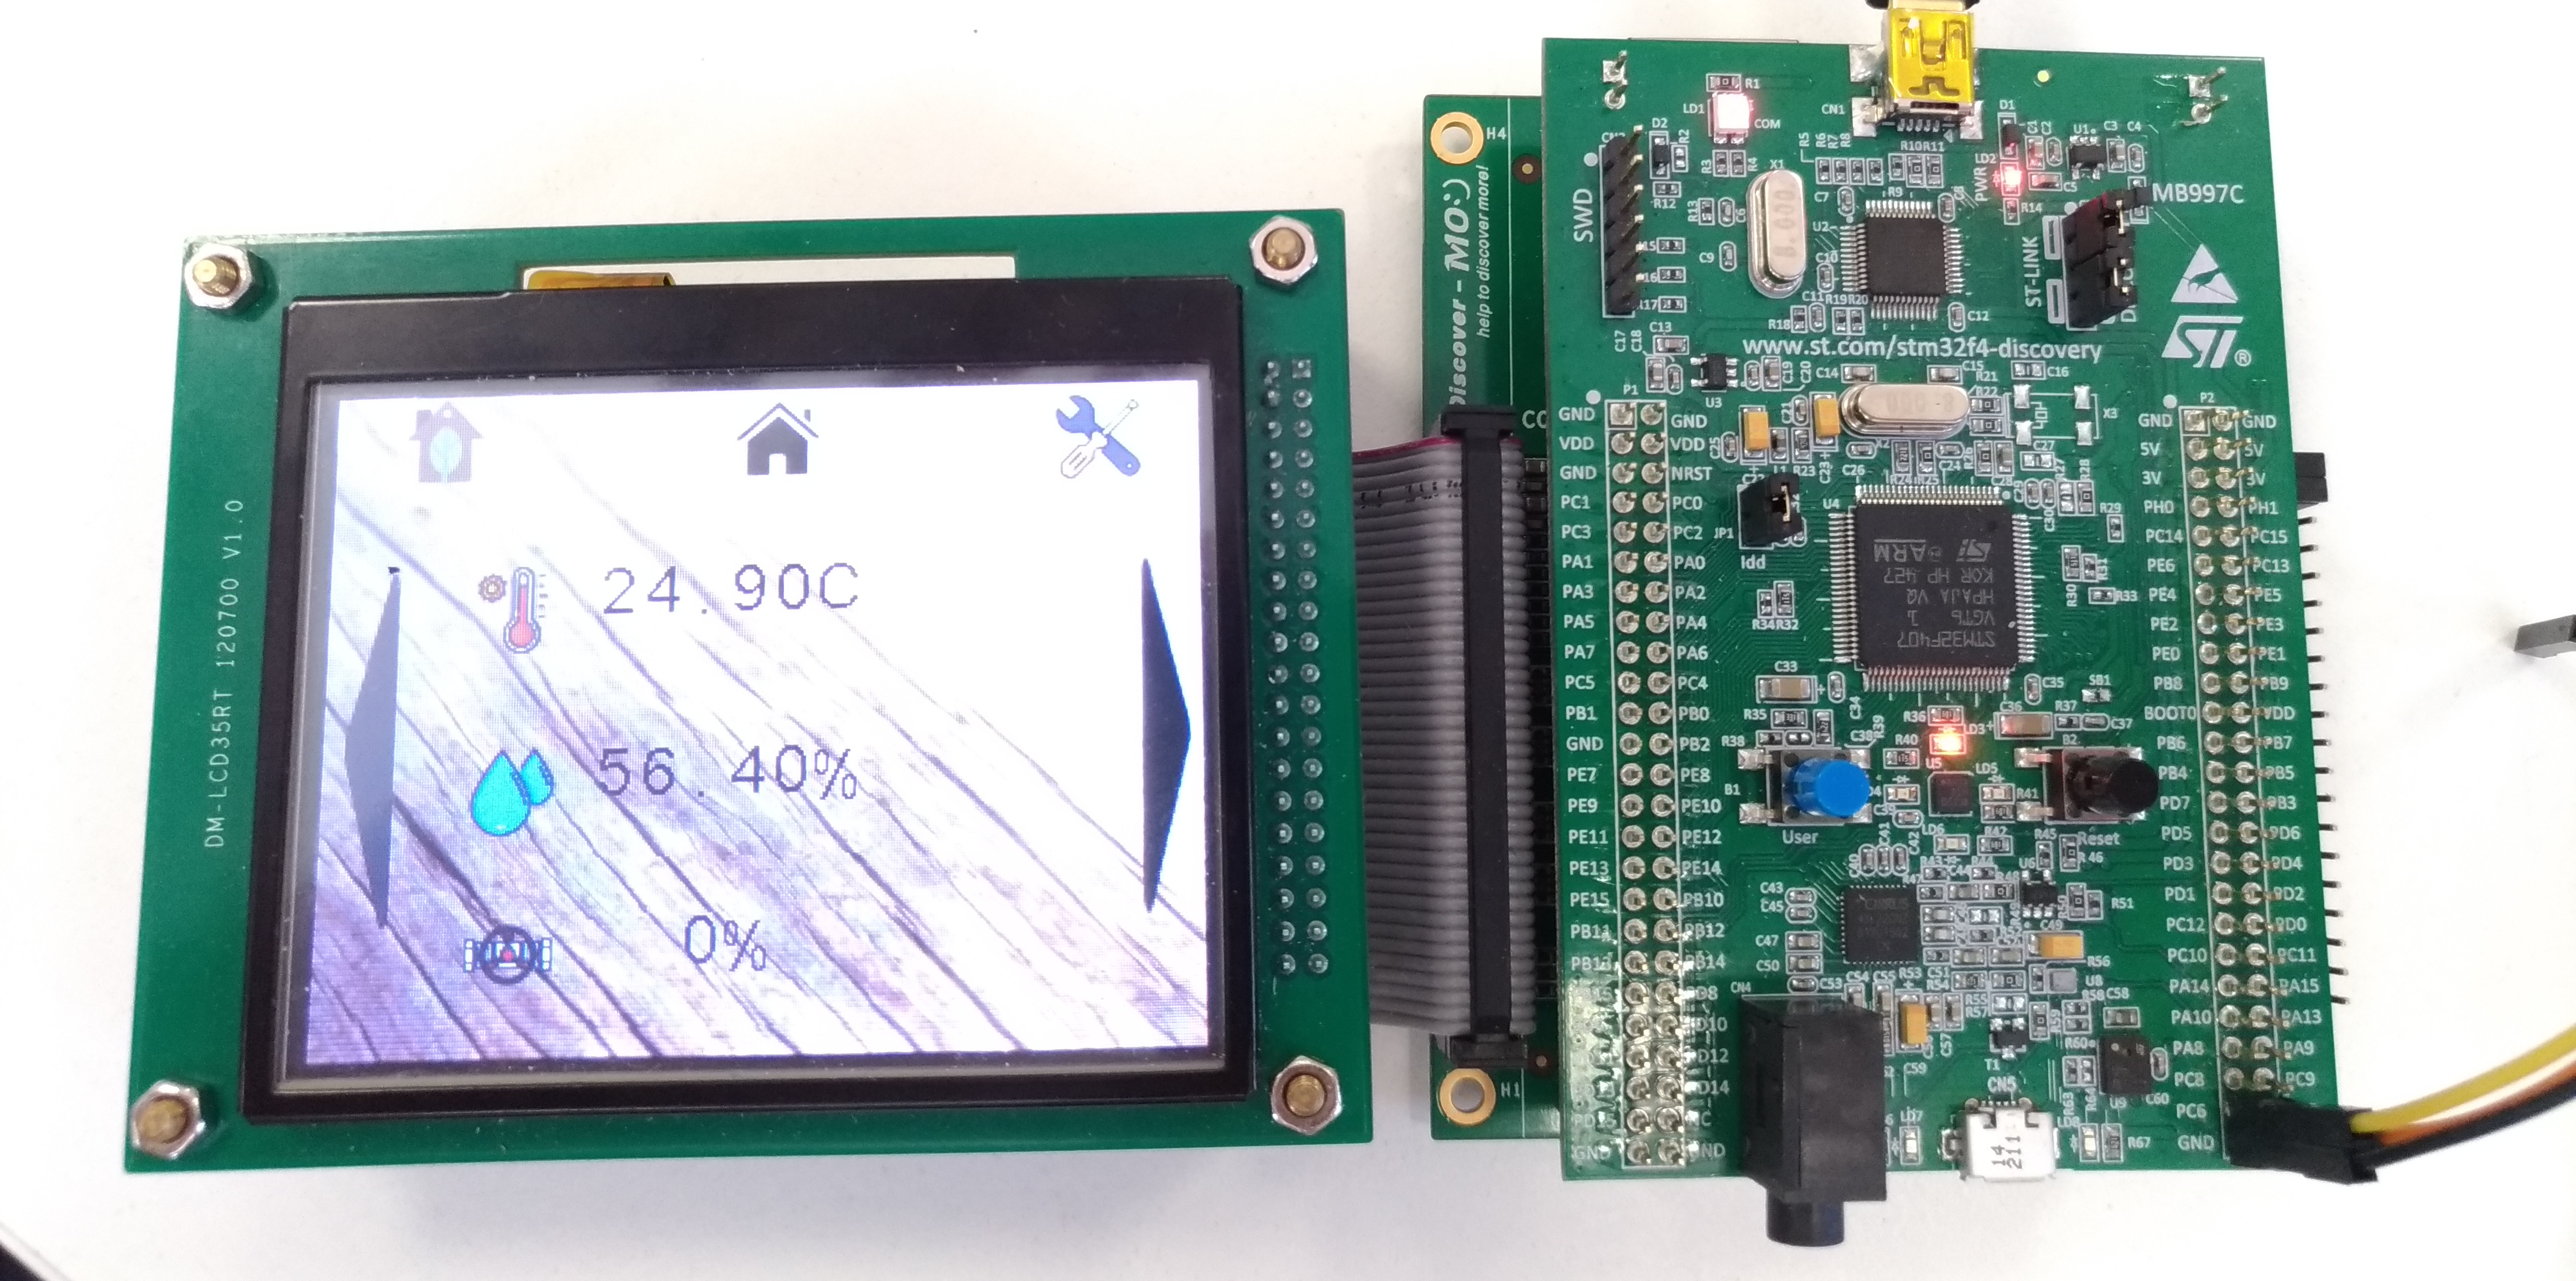
\includegraphics[width=8cm,keepaspectratio]{img/CentralUnit}
	\caption{Central Unit module}
	\label{fig:CentralUnit}
\end{figure}

The module is composed by:
\begin{itemize}
	\item STM32F407VG DISCOVERY powered by ARM Cortex-M4 32-bit
	\item LCD board Touchscreen 3”5
\end{itemize}
In the discovery board are running the \textit{CentralUnit's} tasks on top of Erika RTOS, the systen is composed by three different tasks reported in the table \ref{tab:CU_Tasks}.\\
Whenever a \textit{RoomStatus} message arrives through the \textit{USART} interface, the \textit{CheckMessage} aperiodic task is activated in order to check the message and execute the \textit{RoomManager's} functionalities.\\
The \textit{CheckMessage} task apply a simple JSON compliance test and check each field name and value of the message, then the message is converted in a \textit{RoomStrunct} and the Room's status and \textit{Building} status are updated.\\
While the \textit{CheckMessage} task has the role of processing the incoming \textit{RoomStatus}, the \textit{Polling} task has the role of managing the rooms sending a check message periodically one room after the other, 
if the response \textit{RoomStatus} message doesn't arrive within the next task's job it's considered as an error and the same \textit{RoomRequest} message is sent until a maximum of 3 resend, then the room is marked as crashed.\\
The \textit{Graphic} task has the role to represent the data of the building and for each room depending on the selected page by the user, in the settings page the user is able to set the desired temperature that will be sent starting from the next job of the \textit{Polling} task.\\
\begin{center}
	\begin{tabular}{||c | c | c ||} 
		\hline
		Name 	& Frequency & Priority	\\ 
		\hline
		\textbf{Check Message task}	&	Aperiodic		& 3 	\\ 
		\hline
		\textbf{Polling task}		&	0.2Hz			& 2 	\\ 
		\hline
		\textbf{Graphic task}		&	10Hz			& 1 	\\ 
		\hline
		\textbf{Receiver}			&	USART background		& / 	\\ 
		\hline
	\end{tabular}
	\label{tab:CU_Tasks}
\end{center}

\subsection{Wiring}
\begin{figure}[H]
	\centering
	\includegraphics[width=6cm,keepaspectratio]{img/discovery_board}
	\caption{Discovery board wiring}
	\label{fig:dicovery}
\end{figure}

The module is using the \textit{USART6} of the discovery board to comunicate with the \textit{room} modules, in the following table is reported the configuration of the \textbf{USART6}
\begin{center}
	\begin{tabular}{||c | c | c | c | c | c | c ||} 
		\hline
		USART 	& TX pin 	& RX pin	& baud-rate & Parity Bit & Stop bits & Control Flow \\ 
		\hline
		6		&	PC6		& PC7 		& 9600 & No & 1 & No	\\ 
		\hline
	\end{tabular}
\end{center}

\subsection{Graphic Interface}
The graphic interface is compose by three different screens:
\begin{itemize}
	\item Home screen
	\item Settings screen
	\item Room screen
\end{itemize}
\begin{figure}[H]
	\centering
	\begin{subfigure}{0.4\textwidth} % width of left subfigure
		\includegraphics[width=4cm,keepaspectratio]{img/home_screen}
		\caption{Home screen}
		\label{fig:home_screen}
		\end{subfigure}
	\vspace{1em} % here you can insert horizontal or vertical space
	\begin{subfigure}{0.4\textwidth} % width of right subfigure
		\includegraphics[width=4cm,keepaspectratio]{img/settings_screen}
		\caption{Settings screen}
		\label{fig:settings_screen}
	\end{subfigure}
	\begin{subfigure}{0.4\textwidth} % width of right subfigure
		\includegraphics[width=4cm,keepaspectratio]{img/room_screen}
		\caption{Room screen}
		\label{fig:room_screen}
	\end{subfigure}
\end{figure}
The main page is the \textbf{home screen} reported in \ref{fig:home_screen}, in this page are reported the average values of the building,
If at least one room is marked as \textit{crashed} then a warning appear on the home screen.
If at least one room is in \textit{eco mode} then an \textit{eco} icon is displayed on the home screen.
If the difference between the desired temperature and the actual average temperature is less then 0.5C\degree, the shown termometer icon is hot otherwise cold.
In the \textbf{settings screen} reported in \ref{fig:settings_screen} it is possible to set the desired temperature of the building that is the same for each room.
In the \textbf{room screen} reported in \ref{fig:room_screen} is displayed the status of the selected room, status composed by:
\begin{itemize}
	\item Eco mode (the icon on the top-left of the screen)
	\item Temperature
	\item Humidity
	\item Valve position
	\item Warning (Warning icon between the eco icon and the icon in the top-center)
\end{itemize}
